\section{Top Physics}\label{sec:top-physics}

The top quark is the heaviest particle in the SM. Despite being theorised since 1973, it has not been studied to the same extent as the other fermions and leptons due to its relatively recent discovery in 1995\cite{Quadt}. 
Indirect evidence from electroweak precision data inferred its existence exactly where it was found. 
The strong and weak interactions of the top quark have not been measured to the same extent as the other quarks and leptons.
The strong force is most directly measured in top quark pair production and the weak force through top decay and single top production\cite{Quadt}. 

Many of its properties, stemming from its mass  of $173.44 \pm 0.76 \GeV$ and short lifetime, have no equivalent for the other five quarks\cite{LHC:2014combination}. 
With the mass of the top quark being close to the electroweak symmetry breaking scale, measuring top quark decay and single top quark production provides an excellent probe of the weak interaction and a means to indirectly search for evidence of new physics beyond the SM. 
Unlike the lighter quarks, which are confined to hadronic states due to the strong force, the top quark decays quicker than the strong force’s characteristic time.
As such, it is the only known ``bare'' quark in nature, even if only for a brief amount of time. 
This allows physicists the opportunity to directly observe the spin of a bare quark, rather than the overall spin of a composite hadronic particle, through the spin of its decay products as strong interactions will not have a chance to depolarise it.
Top quarks will also be a significant component of the background for new signal searches in the TeV range, requiring an understanding of this signal in order to find new physics beyond the SM\cite{Quadt}.

Due to the top quark’s large mass, only sufficiently powerful particle colliders can produce them. 
Whilst the Tevatron could produce top quarks, due to the relatively low production rate, and thus statistics, the data which was used to analyse the top quark’s properties was limited.
Because of the LHC’s greater operational energy and integrated luminosity, greater statistics will be available to probe the nature of the top quark\cite{Shibata:2008sy}. 

Top quarks are predominately produced by pair-production through the strong force (Figure~\ref{fig:feyn_ttbar}).

\begin{figure}[htbp]
\begin{center}
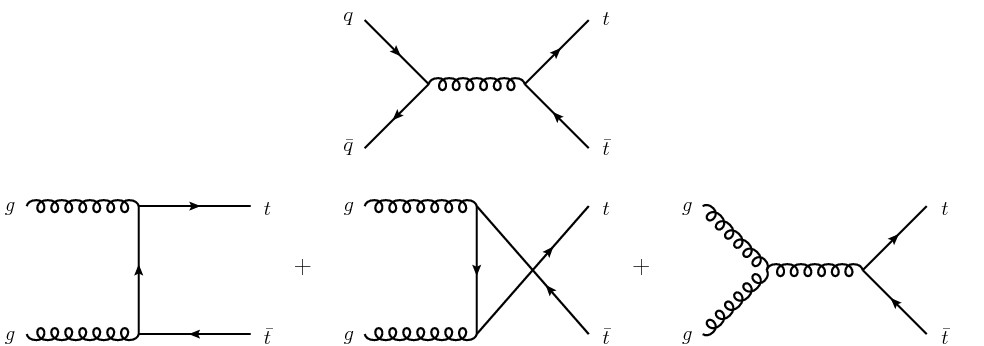
\includegraphics[width=0.97\textwidth]{figs/top-physics/ttbar_feyn.jpg}
\caption{Lowest Order Feynman diagrams contributing to top quark pair production at hadron colliders. Quark-anti quark annihilation is illustrated on the top row and gluon fusion on the bottom . Gluon fusion is the main production mode at the LHC and pair production at the Tevatron.}
\label{fig:feyn_ttbar}
\end{center}
\end{figure}

At the LHC the dominant mode of production is through gluon fusion, with quark-anti quark annihilation and the decay of the neutral photon and $Z^{0}$ bosons having smaller cross-sections\cite{Shibata:2008sy}.

Singly produced top quarks are produced through weak interactions by three differing channels \ref{fig:feyn_singletop}).
Such processes are an excellent probe of the SM as it allows the direct measurement of the $\abs{V_{tb}}$ element of the Cabibbo-Kobayashi-Maskawa (CKM) matrix as the top quark predominately decays to a bottom quark and thus test whether the CKM matrix is indeed unitary as presumed, or otherwise\cite{Shibata:2008sy}.

\begin{figure}[htbp]
\begin{center}
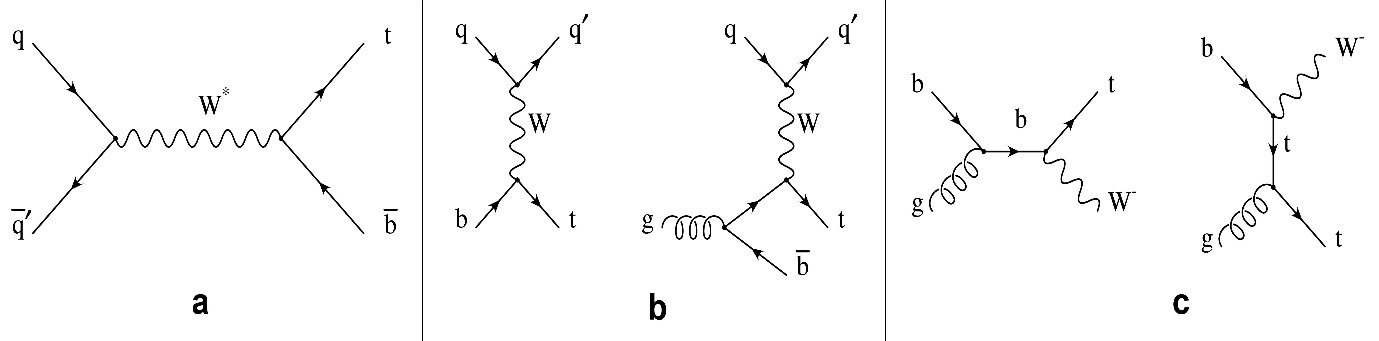
\includegraphics[width=1.00\textwidth]{figs/top-physics/singletop_feyn.jpg}
\caption{Feynman diagrams of single top production channels: a) s-channel; b) t-channel; c) tW-channel.}
\label{fig:feyn_singletop}
\end{center}
\end{figure}

Top quark pair production in association with a $\gamma$, $Z^{0}$, and $W^{\pm}$ vector bosons, are all expected to have a similar cross section and can be used to test the consistency of the SM and search for Beyond the SM (BSM) physics.
These channels, despite their small cross-sections, are important backgrounds which need to be understood in order to be able to probe for new physics with similar or smaller cross sections, such as $\ttbar$H\cite{Khachatryan:2014ewa}.

The production of a single top quark in association with a $Z^{0}$ boson with an additional jet (tqZ), is a single top channel of interest.
This is a rare SM process that is based on single top production in the t-channel. The $Z^{0}$ boson is radiated off one of the quark legs, or from an exchanged W boson (Figure~\ref{fig:feyn_tZq}).
A greater understanding of the behaviour of this background is paramount to searches for BSM physics as this process is an irreducible background for many such searches of new physics (such as for Flavour Changing Neutral Current processes)\cite{Quadt}. 

%\begin{figure}[p]
%\centering
%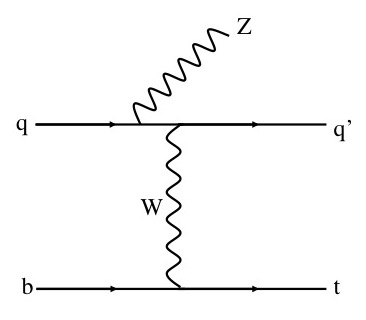
\includegraphics[width=0.47\textwidth]{figs/top-physics/tZq_feyn1.jpg}
%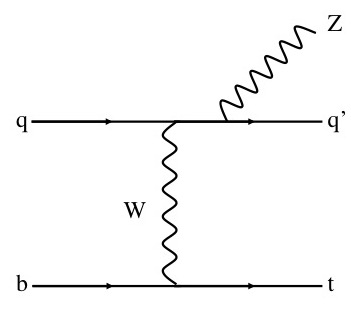
\includegraphics[width=0.47\textwidth]{figs/top-physics/tZq_feyn2.jpg}
%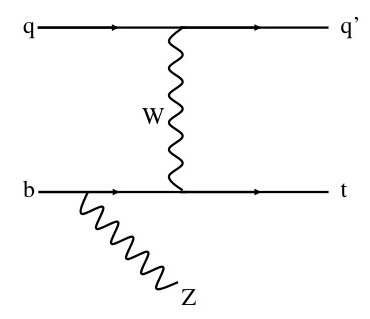
\includegraphics[width=0.47\textwidth]{figs/top-physics/tZq_feyn3.jpg}
%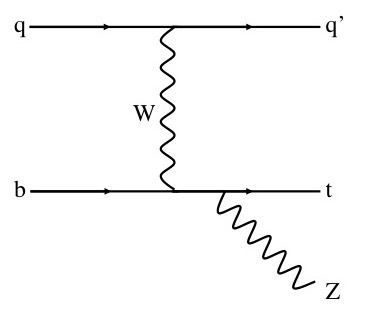
\includegraphics[width=0.47\textwidth]{figs/top-physics/tZq_feyn4.jpg}
%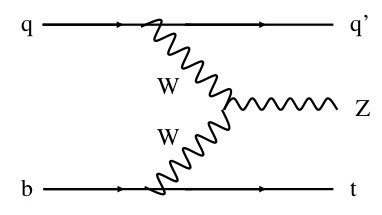
\includegraphics[width=0.47\textwidth]{figs/top-physics/tZq_feyn5.jpg}
%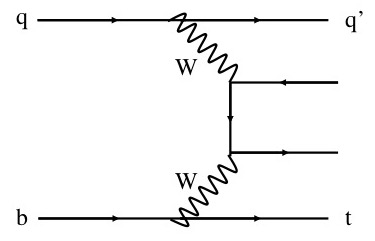
\includegraphics[width=0.47\textwidth]{figs/top-physics/tZq_feyn6.jpg}
%\caption{Leading order tZq production diagrams. Diagram (f) represents the non-resonant contribution to the tqZ process.}
%\label{fig:feyn_tZq}
%\end{figure}

Prior to the first run of the LHC, proton-antiproton data for the top quark was collected at the Tevatron during both Run-I (at a centre-of-mass energy of 1.8 TeV) and Run-II (at a centre-of-mass energy of 1.96 TeV), corresponding to an integrated luminosity of 8.7 \fbinv.
The \ttbar production (di-lepton, lepton+jets and all-jets) cross section was within 9\% of the expected SM result\cite{Lister:2008it} and the measurement of the top quark’s mass had a relative precision of 0.75\%\cite{Group:2009ad}.
The Tevatron also found both the first evidence for the production of single top quarks\cite{Abazov:2006gd} as well as discovering the production channel and from the measured cross-section, both collaborations were able to directly determine the CKM matrix element which describes the Wtb coupling and determine that it had a 95\% confidence level of being consistent with the SM\cite{Aaltonen:2009jj}.

During 2012, $19.7\pm0.5 \fbinv$ at a centre-of-mass energy of 8 TeV (roughly four times larger than the 7 TeV data) was collected by the CMS Collaboration at the LHC. 
Analysis of the top quark pair production cross-section is generally in good agreement with the SM predictions at next-to-next-to-leading order (NNLO). 
The pT spectrum for data for leptons, jets and top quarks however, is softer than the predictions and similarly to CMS measurements at 7 TeV, the NLO+NNLO calculations fails to describe the data for all$ \pT^{\ttbar}$ values\cite{Khachatryan:2015oqa}. 
Measurements of the W boson helicity fractions from the decay of a single top quark, at centre-of-mass energies of 8 TeV, are in agreement with the SM predictions at NNL0  and have a similar precision to the W boson helicity fractions measurements from top quark pair production at 7 TeV at the LHC\cite{Khachatryan:2014vma}.

At the LHC, for proton-proton collisions at 8 TeV the predicted cross-section at next-to-leading order (NLO) for SM tZ production is\cite{Campbell:2013yla}:

\begin{equation}
\sigma(tZ)= 160_{-2}^{+7} (scale)_{-11}^{+11} (PDF)  fb
\sigma(\bar{T}Z)= 76_{-1}^{+4} (scale)_{-5}^{+5} (PDF) fb
\end{equation}

This leads to an overall cross-section of $236_{-16}^{+19}$ fb. 
These cross-sections were determined using the CTEQ6M set of Parton Distribution Functions (PDF)\cite{Pumplin:2002vw}. 
The $\bar{t}$Z cross-section is roughly half that of the tZ cross-section due to the ratio of the up quark PDF to the down quark PDF is circa 0.5 in the x range typical for these processes\cite{Campbell:2013yla}. 
The CMS collaboration have measured the $\ttbar$Z cross-section to be\cite{Khachatryan:2014ewa}

\begin{equation}
\sigma \ttbar Z)= 200_{-70}^{+80} (statistics)_{-30}^{+40} (systematics) fb
\end{equation}

The cross-section between $\ttbar$Z and the sum of the tZ and $\bar{t}$Z cross-sections is comparable as whilst single top + Z processes are electroweak interactions (in contrast to the QCD-induced top quark pair production) they have fewer daughters in the final state and the Z boson condition for $\ttbar$Z considerably reduces the rate\cite{Campbell:2013yla}.
As such, a search for tZ processes should be achievable during CMS Run-1 data. This is supported by CMS’ Run-I results for $\ttbar$Z\cite{Khachatryan:2014ewa}. 
A CMS Analysis Note and a journal paper supporting a three sigma probability of evidence of single top production in association with a Z boson and a jet are currently being produced by the HEP Group at Brunel University London\cite{Sirunyan:2017kkr}.

Until now, the 2012 data taken at 8 TeV, has been used by the research group to analyse these processes.
Following the restart of the LHC after the phase-0 upgrades, new data are anticipated to be available with the increase to a higher centre-of-mass energy and with anticipated luminosities of up to 3000\fbinv\cite{ECFA}. 
Such statistics will be used to gain more precise measurements of top quark pair production and the production of single top quarks and as a result, a better understanding of the underlying processes involved.
